% !TeX root = ../main.tex

\chapter{ROS导航和可佳导航简介}

\section{ROS导航}

ROS(Robot Operating System)是一个开源的专用于机器人软件开发的操作系统。ROS中提供了一个模块化的简单2D导航系统ROS Navigation,其主要架构如图\ref{fig:rosnav}所示。

\begin{figure}[htb]
  \centering
  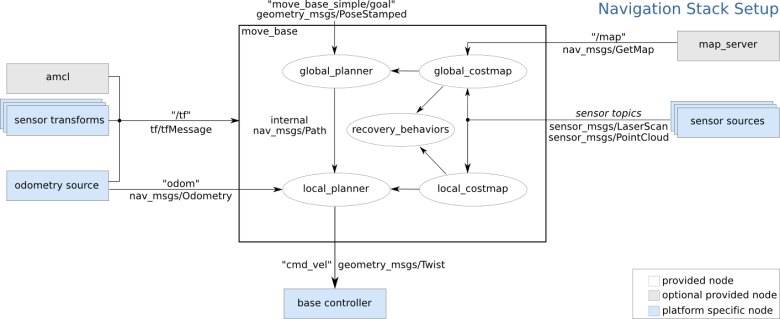
\includegraphics[width=1.1\textwidth]{ROS_navigation_stack.png}
  \caption{ROS导航架构}
  \label{fig:rosnav}
\end{figure}

\subsection{建图}
  包括gmapping\cite{grisetti2007improved}和cartographer\cite{hess2016real}两种方法。

\subsection{定位}
  amcl是有图后的定位模块,使用粒子滤波算法进行对机器人当前位置的估计。

\subsection{costmap}

  地图表示与更新。

\subsection{导航控制}

  导航控制模块即图\ref{fig:rosnav}中的move base模块。包括全局规划器、局部规划器和恢复机制。

\section{可佳导航}

\begin{figure}[htb]
  \centering
  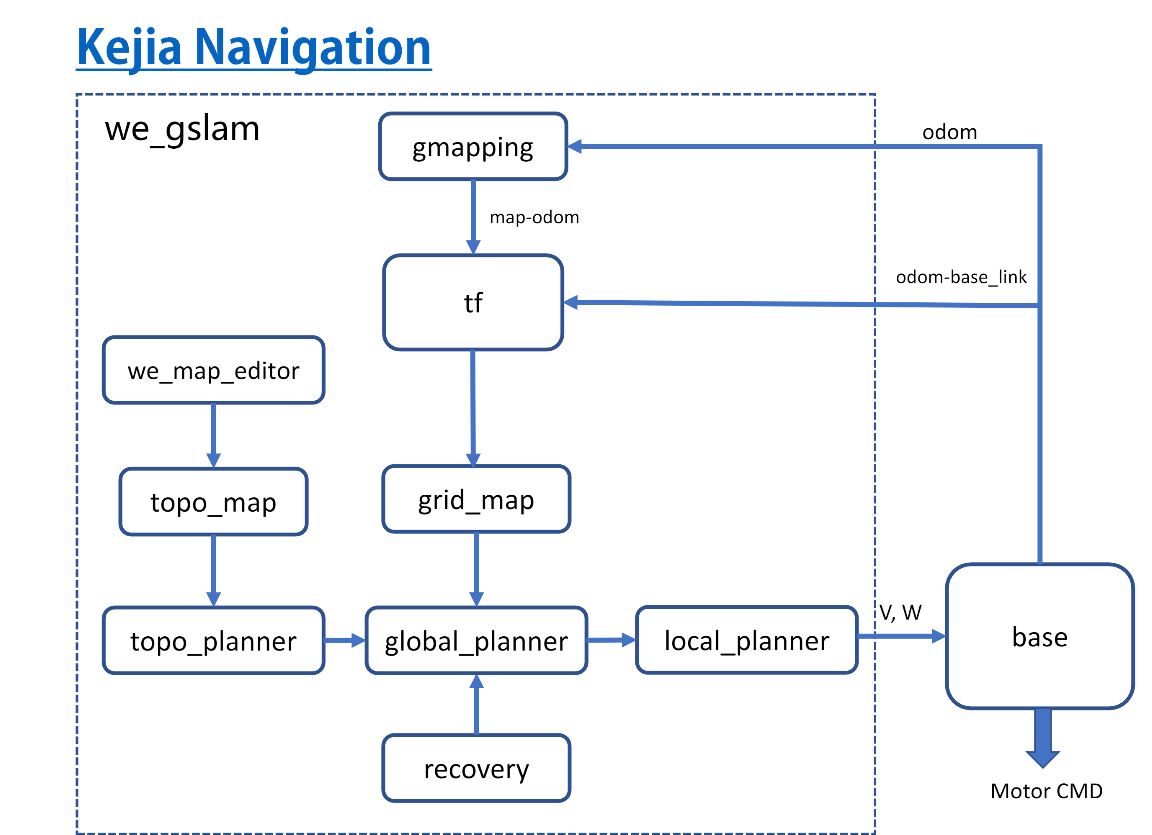
\includegraphics[width=1.1\textwidth]{kejianav.png}
  \caption{可佳导航架构}
  \label{fig:kejianav}
\end{figure}

  可佳导航的架构如图\ref{fig:kejianav}所示。在导航方面,它相对于ROS导航,还加入了拓扑导航。使用VFH(vector field histogram)\cite{borenstein1991vector}进行局部避障。